\documentclass[11pt]{article}
\usepackage[margin=1in]{geometry}
\usepackage{graphicx}
\usepackage{amsmath}
\usepackage{amssymb}
\usepackage{booktabs}
\usepackage{siunitx}
\usepackage{xcolor}
\usepackage{caption}
\usepackage{subcaption}
\usepackage[colorlinks=true,linkcolor=blue!55!black,urlcolor=blue!55!black]{hyperref}
\captionsetup{font=small,labelfont=bf}
\graphicspath{{figs/}}
\newcommand{\um}{\,\mu\mathrm{m}}
\newcommand{\mm}{\,\mathrm{mm}}
\newcommand{\mrad}{\,\mathrm{mrad}}
\sisetup{detect-all}

\title{\vspace{-1.5em}Intrinsic resolution of the MX17 ``M3'' reference telescope and
its pointing uncertainty at the device-under-test\\
\large Four-plane cosmic self-calibration --- June 2026 bench (det3 saturday long run)}
\author{MX17 cosmic-bench analysis}
\date{2026-07-15}

\begin{document}
\maketitle
\vspace{-1.2em}

\begin{abstract}
\noindent The MX17 ``M3'' reference tracker is a genuine four-plane beam telescope in each
coordinate. Using a per-plane reprocessing of the cosmic data we measure the intrinsic
resolution of its eight strip planes by the geometric-mean unbiased-residual method, bound the
multiple-scattering (MS) contribution, and propagate the resulting \emph{pointing uncertainty}
to the device-under-test (DUT) planes at $z=232$ and $702\mm$. The reference planes resolve to
$\sigma_X\!\approx\!0.41\mm$ (uniform) and $\sigma_Y\!\approx\!0.45$--$0.51\mm$. The telescope
points to the DUT with a Gaussian-core error of $0.22\mm$ (mid-gap, $z=702$) to $0.27\mm$
($z=232$); this is $23$--$33\%$ of the variance of the measured DUT residual. Deconvolving it
gives a DUT intrinsic resolution of $\sigma_\mathrm{DUT}\approx0.40\mm$. Inside the tracking
volume the reference \emph{always} out-points the DUT in the core; a DUT can only beat the
reference in extrapolation or against the MS-scattered reference tail.
\end{abstract}

\section{Why the measurement is possible: geometry}
The reference tracker consists of \textbf{eight MultiGen-v2 strip planes in four stations}, each
station carrying one $X$ and one $Y$ plane (Fig.~\ref{fig:geom}). Consequently each coordinate
is an \emph{independent four-point straight-line fit} --- a four-plane telescope --- so the
classic ``fit three, predict the fourth'' self-calibration applies. Geometrically the stations
form two tight \textbf{doublets} ($\Delta z\!\approx\!117$/$120\mm$) separated by a
$\sim\!1041\mm$ lever arm; the DUT slots sit \emph{interpolated} in the gap.

\begin{figure}[h]
\centering
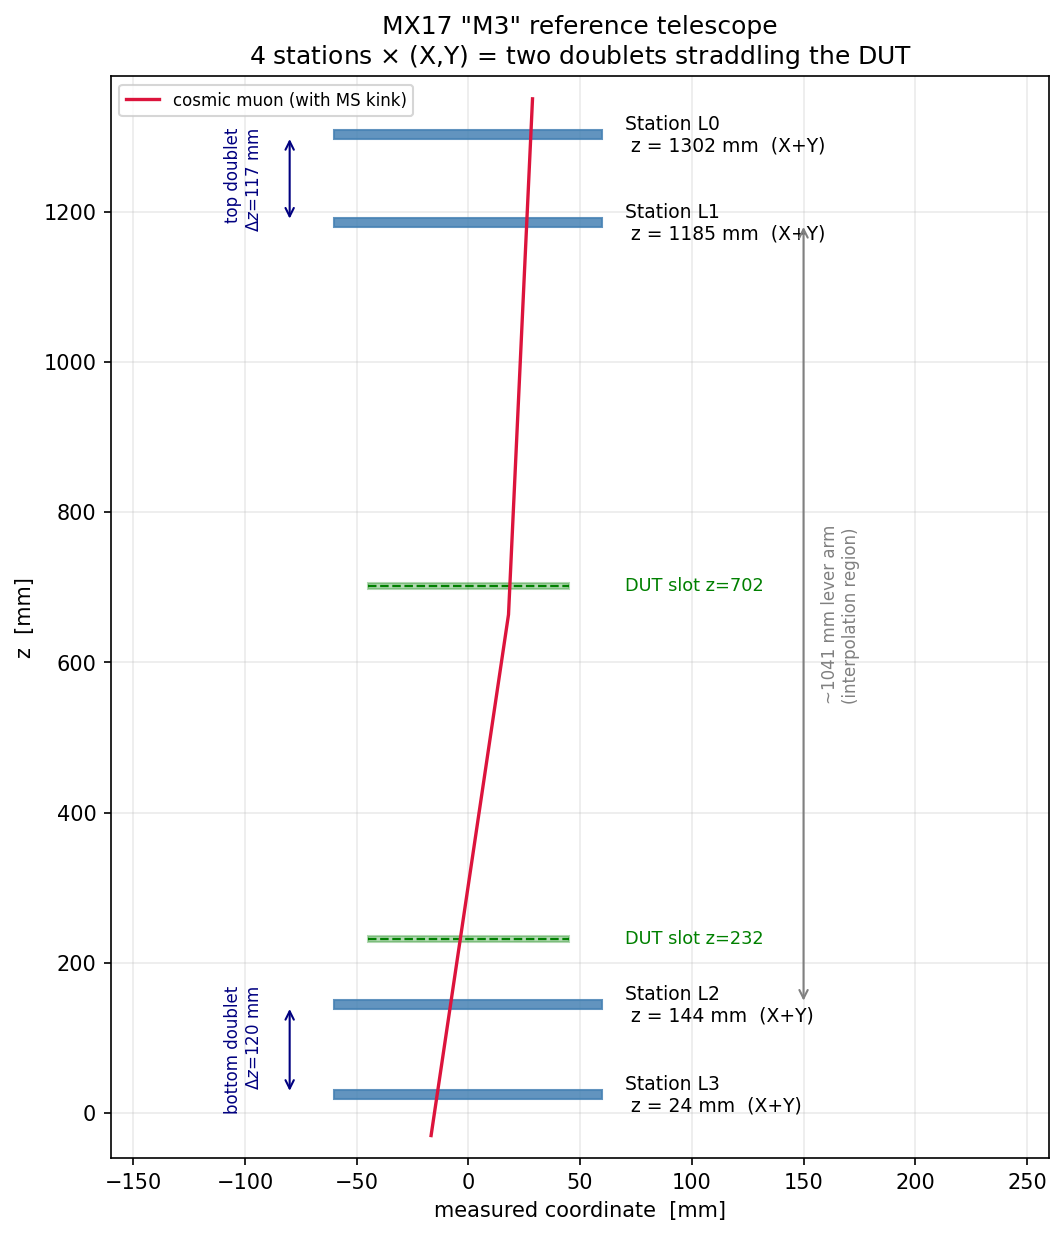
\includegraphics[width=0.62\textwidth]{geometry.png}
\caption{The M3 reference telescope: four $X{+}Y$ stations at $z=24,144,1185,1302\mm$ forming a
bottom and a top doublet, with the two DUT slots ($z=232,702\mm$) interpolated inside the
$\sim\!1\mm$-material gap. A cosmic muon with a small multiple-scattering kink is sketched.}
\label{fig:geom}
\end{figure}

\section{Data and method}
\textbf{Data.} det3 weekend ``saturday'' long run (resist $490$\,V, drift $1000$\,V), files
0--3, locally reprocessed after patching the tracking producer to emit the per-station cluster
positions used in each fit ($41\,455$ rays). A recomputation of $\sum\text{residual}^2$ from
the emitted positions reproduces the producer's $\chi^2$ to a median $7\times10^{-4}\mm^2$,
confirming they are exactly the fit inputs. All widths below are robust \textbf{Gaussian-core}
fits (iterative $\pm2.5\sigma$) so the MS tails do not bias the intrinsic estimate; only
four-hit ($\mathrm{NClus}=4$) single-track events are used.

\textbf{Per-plane intrinsic resolution.} For each plane $k$ we form the \emph{biased} residual
(all four planes in the fit, width $\sigma_{\mathrm{incl},k}$) and the \emph{unbiased} residual
(fit the other three, predict $k$, width $\sigma_{\mathrm{excl},k}$). The intrinsic width is the
geometric mean
\begin{equation}
\sigma_k=\sqrt{\sigma_{\mathrm{incl},k}\,\sigma_{\mathrm{excl},k}},
\qquad\text{since}\quad
\sigma_{\mathrm{incl}}^2=\sigma_k^2(1-h_{kk}),\;\;
\sigma_{\mathrm{excl}}^2=\frac{\sigma_k^2}{1-h_{kk}},
\end{equation}
so the leverage/geometry factor $h_{kk}$ cancels exactly. (The alternative simultaneous
unbiased-variance solve is numerically singular here, condition number $\sim\!10^{16}$, because
the within-doublet leave-one-out coefficients diverge --- hence the geometric mean.)

\textbf{Pointing.} The reconstruction fits all four planes unweighted, so the predicted position
at any $z$ is $\hat y(z)=\sum_k g_k(z)\,y_k$ with purely geometric coefficients $g_k(z)$, and the
pointing uncertainty is
\begin{equation}
P(z)=\sqrt{\textstyle\sum_k g_k(z)^2\,\sigma_k^2}.
\end{equation}
The DUT intrinsic resolution follows by quadrature subtraction,
$\sigma_\mathrm{DUT}=\sqrt{\sigma_\mathrm{resid}^2-P(z_\mathrm{DUT})^2}$.

\section{Results}

\subsection{Per-plane intrinsic resolution}
\begin{table}[h]
\centering
\small
\begin{tabular}{lccc@{\hskip 2em}lccc}
\toprule
plane & $\sigma_\mathrm{incl}$ & $\sigma_\mathrm{excl}$ & $\boldsymbol{\sigma_k}$ &
plane & $\sigma_\mathrm{incl}$ & $\sigma_\mathrm{excl}$ & $\boldsymbol{\sigma_k}$\\
 & ($\um$) & ($\um$) & ($\boldsymbol{\um}$) &
 & ($\um$) & ($\um$) & ($\boldsymbol{\um}$)\\
\midrule
$X$ L0 & 278 & 618 & \textbf{415} & $Y$ L0 & 343 & 762 & \textbf{511}\\
$X$ L1 & 304 & 553 & \textbf{410} & $Y$ L1 & 373 & 679 & \textbf{503}\\
$X$ L2 & 304 & 552 & \textbf{409} & $Y$ L2 & 331 & 600 & \textbf{445}\\
$X$ L3 & 275 & 613 & \textbf{411} & $Y$ L3 & 307 & 683 & \textbf{458}\\
\bottomrule
\end{tabular}
\caption{Per-plane intrinsic resolution (geometric mean). The four $X$ planes are uniform at
$\sigma_X\approx0.41\mm$; independent cross-check assuming a single common $\sigma$ gives
$411.2\um$ vs the $411.3\um$ geometric-mean average --- agreement to $0.1\um$. The $Y$ planes
are $0.45$--$0.51\mm$, worse in the resistive charge-spreading direction.}
\label{tab:sigma}
\end{table}

\begin{figure}[h]
\centering
\begin{subfigure}{0.49\textwidth}
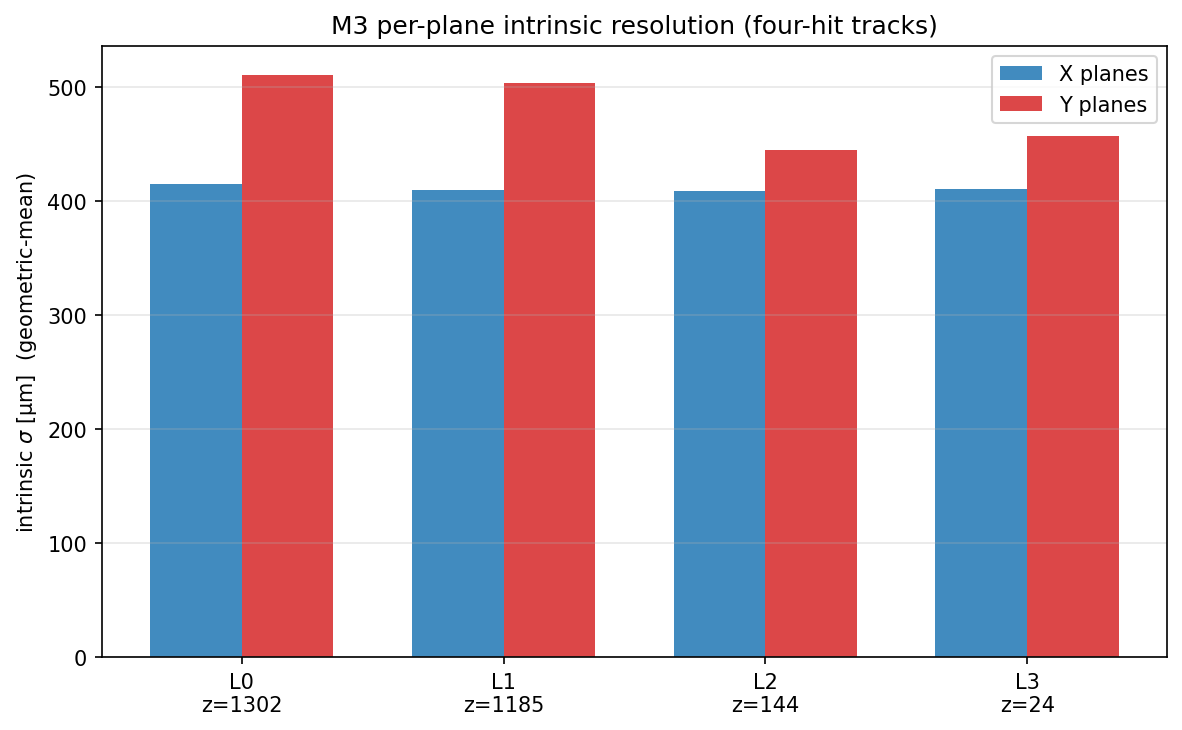
\includegraphics[width=\linewidth]{sigma_per_plane.png}
\end{subfigure}
\hfill
\begin{subfigure}{0.49\textwidth}
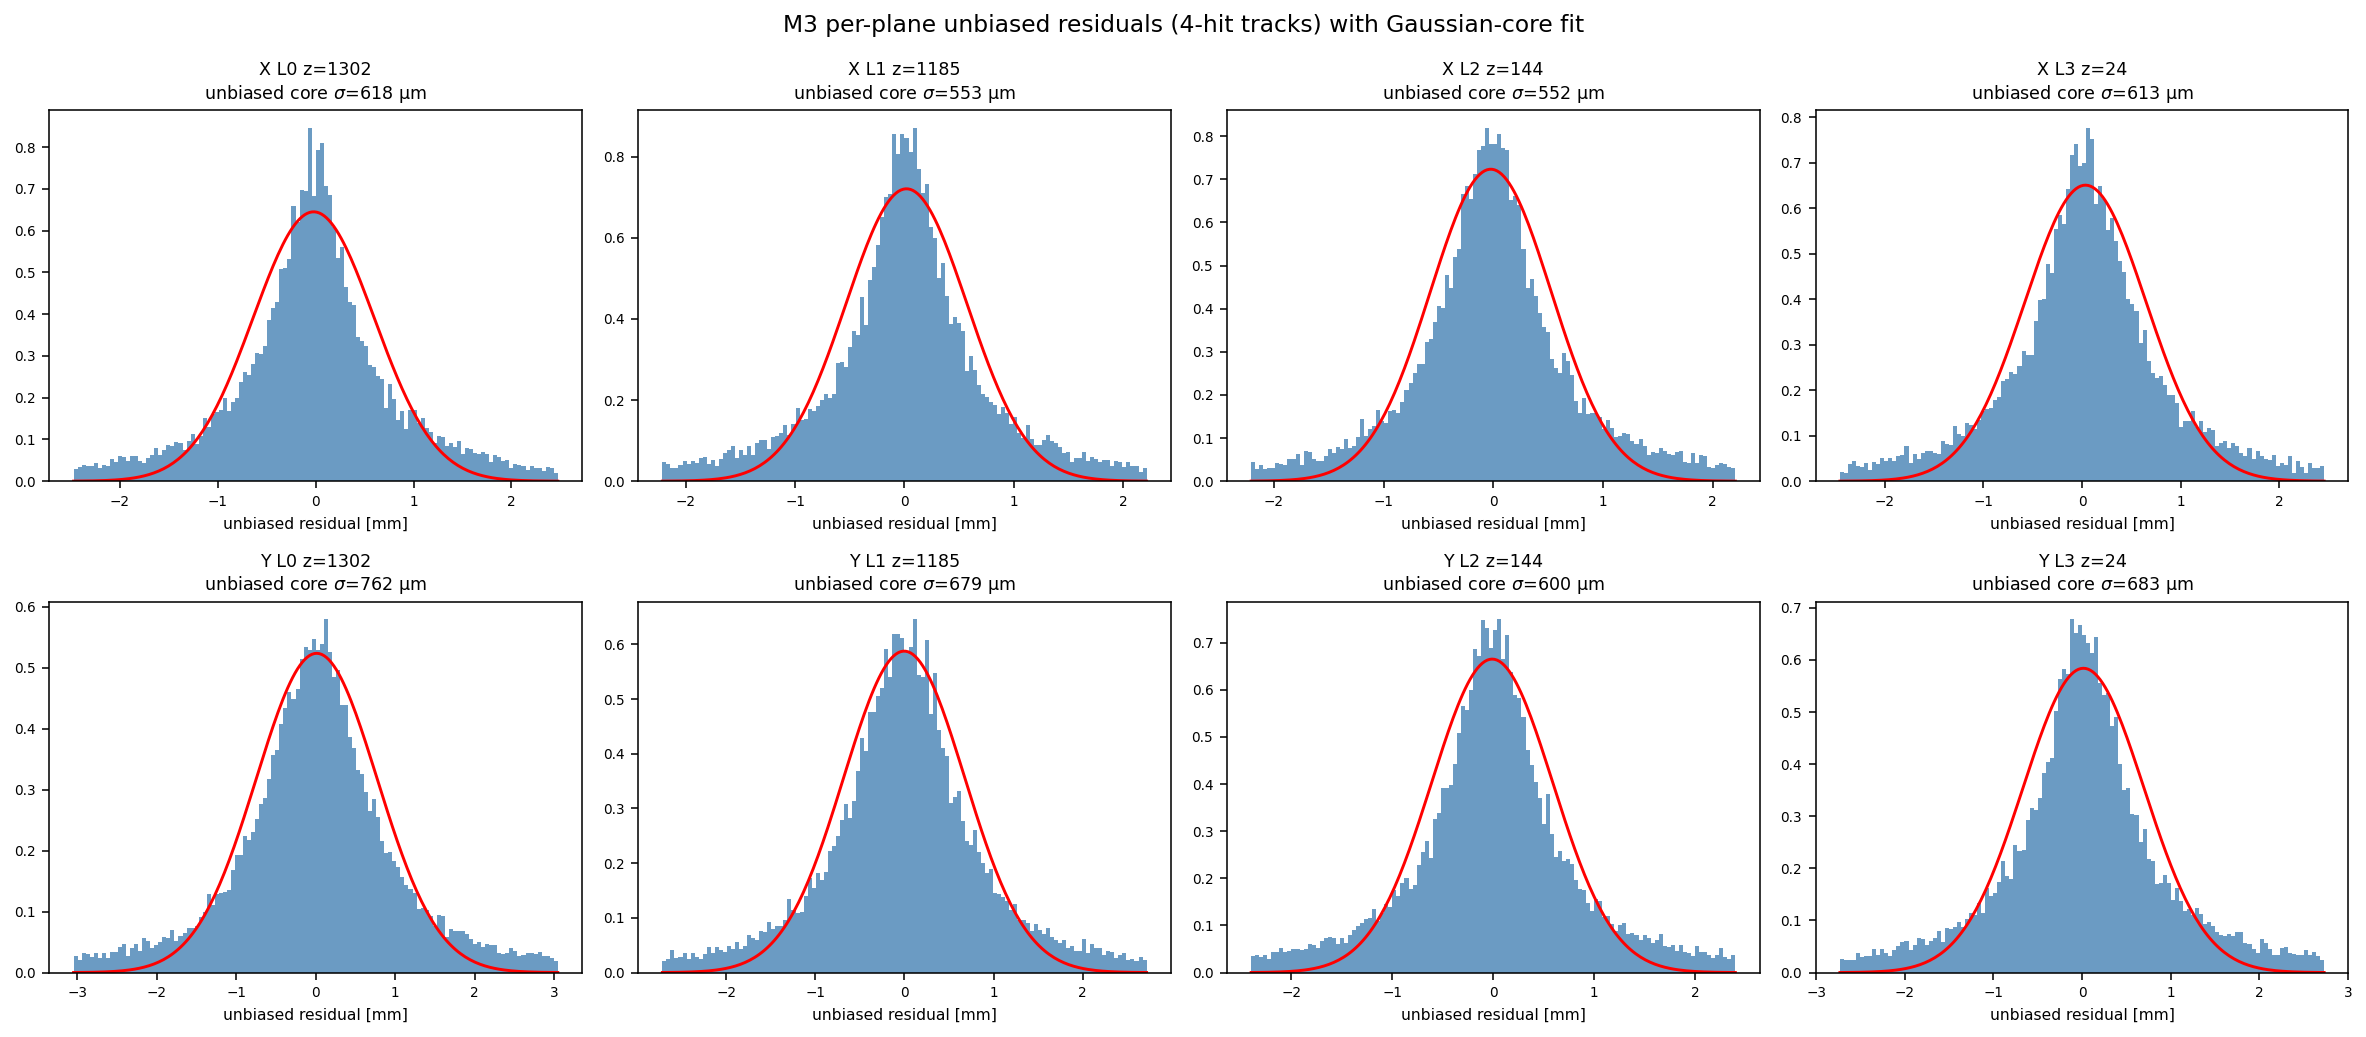
\includegraphics[width=\linewidth]{residuals_per_plane.png}
\end{subfigure}
\caption{Left: per-plane intrinsic $\sigma$. Right: unbiased residuals with Gaussian-core fits;
the peaked cores sit on non-Gaussian multiple-scattering tails.}
\label{fig:res}
\end{figure}

\subsection{Multiple scattering}
The inter-doublet kink gives $\sigma(\Delta\text{slope})=7.4\mrad$ ($X$) against a
resolution-only expectation of $6.9\mrad$, i.e.\ an excess
$\theta_\mathrm{MS}\approx2.6\mrad$ ($X$; $5.0\mrad$ for the noisier $Y$). The Highland estimate
for the rough material budget ($x/X_0\approx0.023$) is $1.8\mrad$ at $1$\,GeV and $0.6\mrad$ at
$3$\,GeV, so the measured core kink is consistent with a soft-plus-hard cosmic mix. Because the
$\sim\!7\mrad$ slope resolution dominates the kink, MS is a sub-dominant term, and it enters the
DUT as the residual \emph{tails} (Fig.~\ref{fig:res}, right), not as core broadening. The
core $\sigma_k$ and $P(z)$ are therefore MS-free by construction.

\subsection{Pointing at the DUT and the crossover}
\begin{table}[h]
\centering
\small
\begin{tabular}{cccccc}
\toprule
$z$ (mm) & $P_X$ ($\um$) & $P_Y$ ($\um$) & $\boldsymbol{P_\mathrm{M3}}$ ($\boldsymbol{\um}$)
 & $\boldsymbol{\sigma_\mathrm{DUT}}$ ($\boldsymbol{\um}$) & ref.\ share of resid.\ var.\\
\midrule
232 (bottom slot) & 255 & 282 & \textbf{269} & \textbf{386} & 33\,\%\\
702 (\emph{sat det3}) & 206 & 242 & \textbf{224} & \textbf{413} & 23\,\%\\
\bottomrule
\end{tabular}
\caption{Reference pointing at the DUT slots (deconvolving the measured DUT core residual
$0.47\mm$ at the $\chi^2<1\,\&\,\mathrm{NClus}=4$ recipe). Pointing is best mid-gap, near the
telescope centroid $\bar z=664\mm$. The deconvolved DUT intrinsic resolution is
$\sigma_\mathrm{DUT}\approx0.40\mm$.}
\label{tab:point}
\end{table}

\begin{figure}[h]
\centering
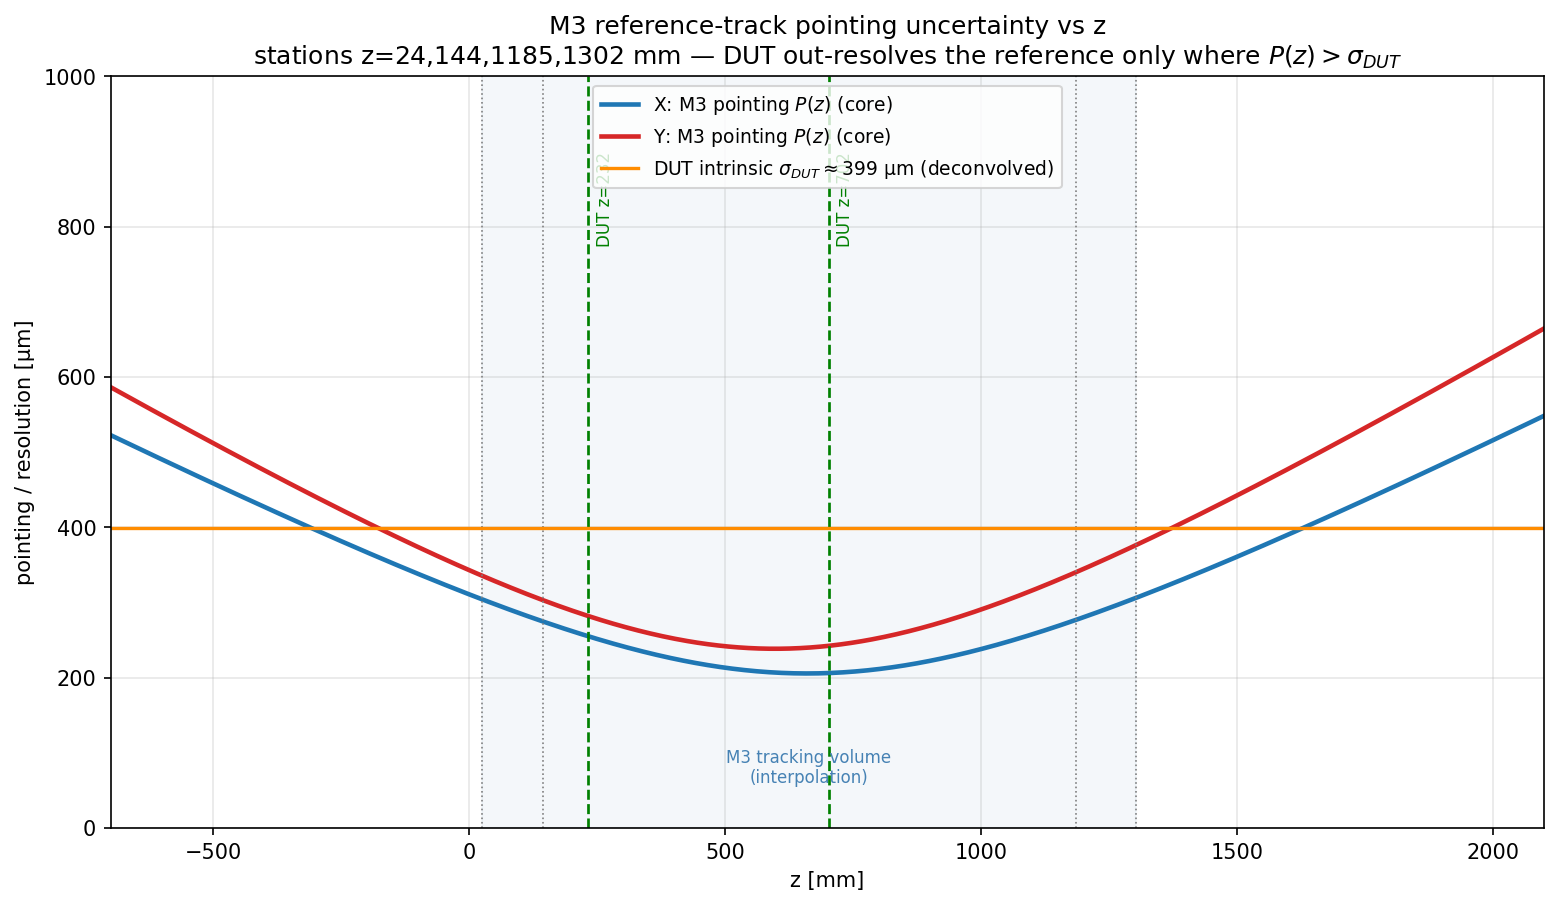
\includegraphics[width=0.78\textwidth]{pointing_vs_z.png}
\caption{Reference-track pointing uncertainty $P(z)$ (Gaussian core). It is minimized near the
telescope centroid and rises steeply outside the stations. The DUT out-resolves the reference
only where $P(z)>\sigma_\mathrm{DUT}$ (orange): above $z\approx1.6$\,m or below
$z\approx-0.3$\,m --- i.e.\ never between the stations.}
\label{fig:point}
\end{figure}

The reference pointing crosses $\sigma_\mathrm{DUT}\approx0.40\mm$ only in the extrapolation
regions ($z\gtrsim1.6$\,m or $z\lesssim-0.3$\,m for $X$; $1.37$\,m / $-0.18$\,m for $Y$).
\textbf{Inside the entire tracking volume $24\le z\le1302\mm$ the reference out-points the DUT}
($P\approx0.21$--$0.28\mm<\sigma_\mathrm{DUT}$).

\section{What this means for DUT analyses}
\begin{itemize}\itemsep2pt
\item The M3 reference points to the DUT with a core $\sigma\approx0.22\mm$ ($z=702$) /
$0.27\mm$ ($z=232$) --- contributing $23$/$33\%$ of the measured DUT residual \emph{variance}.
It is real but sub-dominant in the core; the DUT's own $\approx0.40\mm$ dominates.
\item Report the DUT intrinsic as $\sigma_\mathrm{DUT}=\sqrt{\sigma_\mathrm{resid}^2-P_\mathrm{M3}^2}$,
using $P_\mathrm{M3}=0.22\mm$ at $z=702$.
\item The reference is \emph{not} the core bottleneck --- its \emph{tails} (MS-scattered, low-$p$
muons) are. Tightening the M3 $\chi^2$ removes those and shrinks the residual, but there is no
core gain below $P_\mathrm{M3}$; the DUT resolution is the floor.
\item In the present geometry a DUT never out-resolves the core reference between the stations.
Measuring a sub-$0.2\mm$ DUT would require a $\sigma$-weighted/GBL M3 fit, exploiting the
low-$P$ mid-gap, or an independent higher-resolution reference.
\end{itemize}

\paragraph{Caveats.} The DUT residual ($0.47\mm$) is an external input; a direct join of the
reprocessed rays to the det3 hits would close it self-consistently. The producer fit is
unweighted, so $P(z)$ is the as-reconstructed (slightly conservative) value. $\theta_\mathrm{MS}$
is a core-level estimate, not a spectrum unfold. Numbers are one run / one gas point.

\end{document}
